\documentclass[11pt]{article}
\usepackage[margin=1in]{geometry}
\usepackage[T1]{fontenc}
\usepackage{mathptmx}
\usepackage[scaled=0.92]{helvet}
\renewcommand{\ttdefault}{txtt}
\usepackage{microtype}
\usepackage{amsmath,amssymb,amsthm}
\usepackage{graphicx}
\usepackage{booktabs}
\usepackage{tabularx}
\usepackage[numbers,sort&compress]{natbib}
\usepackage{xcolor}
\usepackage[colorlinks=true,linkcolor=blue!50!black,citecolor=blue!50!black,urlcolor=blue!50!black]{hyperref}
\hypersetup{pdftitle={A Missing Sign Symmetry Accounts for the Linear-Mode-Connectivity Barrier in Minimal-Width Sigmoid Networks},pdfauthor={Mrigesh Lakhanpal},pdfkeywords={linear mode connectivity, permutation symmetry, sign flips, sigmoid networks, loss landscape}}
\usepackage{caption}
\usepackage{float}
\usepackage{enumitem}
\setlist{itemsep=2pt,topsep=4pt}
\captionsetup{font=small,labelfont=bf}

\newtheorem{proposition}{Proposition}
\newtheorem{lemma}{Lemma}
\pagestyle{empty}
\newcommand{\md}[1]{\textsf{#1}}
\newcommand{\eps}{\varepsilon}


\title{\textbf{A Missing Sign Symmetry Accounts for the\\ Linear-Mode-Connectivity Barrier in Minimal-Width Sigmoid Networks}}
\author{Mrigesh Lakhanpal\\
\small \texttt{mrigeshlakhanpal4@gmail.com}\\
\small ORCID: \href{https://orcid.org/0009-0007-9539-9091}{0009-0007-9539-9091}}
\date{October 2026 \quad (preprint, v2.1.3)\\[2pt] \footnotesize This work is licensed under a Creative Commons Attribution 4.0 International license (CC BY 4.0).}

\begin{document}
\maketitle
\thispagestyle{empty}

\begin{abstract}
\noindent
On two-dimensional tasks with separable labels and a convex-polygon positive region, permutation alignment fails to linearly connect independently trained one-hidden-layer sigmoid networks of minimal width. Ainsworth et al.\ left open whether matching fails on thin models or ``some form of invariance other than permutation symmetries'' is at play; Benzing et al.\ noted that deciding this requires an exhaustive search. For irreducible one-hidden-layer sigmoid networks, the exact symmetry group (permutations and sign flips, $2^h h!$ elements at width $h$) is known and small enough to search exhaustively. In Study~1 (one task, width~3, 11 pairs), permutation matching left a median training-error barrier of 17.95 points, sign-aware matching 0.00, and a post-hoc search over all 48 symmetries at most 0.11. Study~2, publicly pre-registered, added four polygons (3--6 edges; 100--120 seeds per task) and tested all five tasks at their measured minimal widths (3 or 4 units at a 2\% error tolerance). Every pre-registered test of the main claim passed on all five: in pairs needing a flip, the best permutation left a median of 9.95--21.65 points, the full search an upper quartile of at most 0.13 (165 pairs), and the ordering held under training error, test error, raw and calibrated loss. The claim fails for one task at each sensitivity threshold (1\%, 5\%). In exploratory analysis, the 157 pairs that learned the same decision lines kept at most 0.21 points; the 8 that did not, 2.38--9.58. A pre-registered prediction of barrier size from the weights failed for error barriers ($\rho = 0.007$), which saturate; an exploratory loss-based re-test gave $\rho = 0.86$ (calibrated: 0.65). ReLU networks have no sign flip and remain open.
\par\medskip\noindent\textbf{Keywords:} linear mode connectivity; permutation symmetry; sign-flip symmetry; sigmoid networks; loss landscape; model merging
\end{abstract}

\section{Introduction}

Two networks trained from different random initializations usually reach similar accuracy and are often joined by curved paths of low loss~\cite{garipov2018loss,draxler2018essentially}, yet the straight line between their weights typically passes through a region of high loss. Entezari et al.~\cite{entezari2022role} conjectured that most of this barrier is an artifact of permutation symmetry: reorder the hidden units of one network appropriately, and SGD solutions become linearly mode connected~\cite{frankle2020linear}. Ainsworth et al.~\cite{ainsworth2023git} gave strong evidence for wide networks, reaching zero-barrier connections between independently trained ResNets once they were wide enough. In narrow networks, however, permutation alignment does not remove the barrier, and the cause has not been established. Ainsworth et al.\ write that their result ``suggests that either our permutation selection methods are failing to find satisfactory permutations on thinner models or that some form of invariance other than permutation symmetries must be at play in the thin model regime''~\cite[Section~5.3]{ainsworth2023git}, and they conjecture that permutation symmetries are ``a necessary piece, though not a complete picture''~\cite[Section~7]{ainsworth2023git}. Benzing et al.\ observe the same failure in narrow fully connected networks and add that ``a thorough falsification of the hypothesis in narrower networks would require an exhaustive (and therefore infeasible) search over the space of permutations''~\cite[Section~3.1]{benzing2022random}. Entezari et al.\ note that small networks lie outside the scope of their conjecture~\cite[Section~3.4]{entezari2022role}.

The failure also appears beyond fully connected ReLU networks: on independently trained $\tanh$ CNNs with 16 channels per layer, Boufalis et al.\ find that permutation-only Git Re-Basin ``still faces a significant performance barrier, with accuracy dropping sharply at the midpoint'', which they relate to limited width and to the limits of weight matching~\cite[Section~5.2]{boufalis2025symmetry}. A missing sign symmetry may contribute to that barrier; their experiments do not isolate it, and CNNs are outside the scope of this study. The thin models of Ainsworth et al.\ are ReLU networks; this paper answers the sigmoid analogue of their question, and the ReLU case remains open.

In general this question is difficult to settle, because the complete symmetry group of a network is either unknown or too large to search. One-hidden-layer sigmoid networks are an exception. For irreducible networks of this kind, the only exact symmetries are permutations of the hidden units and sign flips of individual units, which follow from $\sigma(-z) = 1 - \sigma(z)$~\cite{sussmann1992uniqueness,vlacic2020affine}. The group has $2^h h!$ elements, only 48 at width $h=3$, so the two explanations, \emph{matching failed} and \emph{another symmetry is involved}, can be told apart by trying every element.

This study exploits that exception, using two-dimensional tasks whose decision region is a convex polygon, so that every learned feature of an independently trained network is a line that can be drawn. To my knowledge, this is the first study of linear mode connectivity in neural networks that searches the complete group of exact symmetries exhaustively, verifies irreducibility so that the group is known to be complete, and separates the barrier left by permutations alone from that left by permutations with sign flips; its scope is one-hidden-layer sigmoid networks. Sign-aware alignment itself is not new~\cite{pittorino2022deep,boufalis2025symmetry}, and an analogous permutation/flip decomposition has been reported for soft tree ensembles~\cite{kanoh2025linear} (Section~\ref{sec:background}). The contributions are:

\begin{enumerate}[leftmargin=*]
\item \textbf{A missing symmetry in the matcher, not a failed search, explains the barrier at width~3} (Study~1, pre-registered; Section~\ref{sec:flips}). On the coffee task (23 of 40 networks met the inclusion rule, 11 pairs), permutation matching leaves a median training-error barrier of 17.95 points, and exhaustive search over the 6 permutations still leaves 17.88. Matching with sign flips removes it (median 0.00), and an exhaustive search over all 48 symmetries leaves at most 0.11 points (post-hoc analysis, rule fixed before the search ran; Section~\ref{sec:b1}).
\item \textbf{The result generalizes across tasks and minimal widths} (Study~2, publicly pre-registered; Section~\ref{sec:v2}). On five tasks with measured minimal widths 3 and 4, every pre-registered test of the main claim (H4a--c and H5) passed at the main 2\% threshold, and the ordering tested by H5 held under all four barrier measures; at each sensitivity threshold (1\%, 5\%) the claim failed for one task. The minimal width depends on the error tolerance. In exploratory analysis, the residual stayed below $\eps$ in 328 of the 331 distinct pairs that learned the same lines.
\item \textbf{Negative results.} The pre-registered prediction that the weights alone predict the size of the barrier failed in error terms, because the error barrier saturates at the trivial classifier. In loss terms it held in an exploratory re-test (Section~\ref{sec:v2h7}). The sensitivity runs contain two task--tolerance combinations where the claim fails.
\end{enumerate}

\noindent In both studies the hypotheses were fixed before any network was trained. The Study~2 rules were committed to a public repository before training began, and its trained models were frozen with SHA-256 fingerprints before any barrier was computed. Every decision taken after seeing results is labelled. One command, including tests, rebuilds every Study~1 result except the optional exhaustive search in about 87 minutes on a laptop CPU and reproduces the main result files byte for byte on the same machine; re-running the Study~2 analysis from the frozen models also reproduces its result files byte for byte (Reproducibility statement).

\begin{figure}[t]
\centering
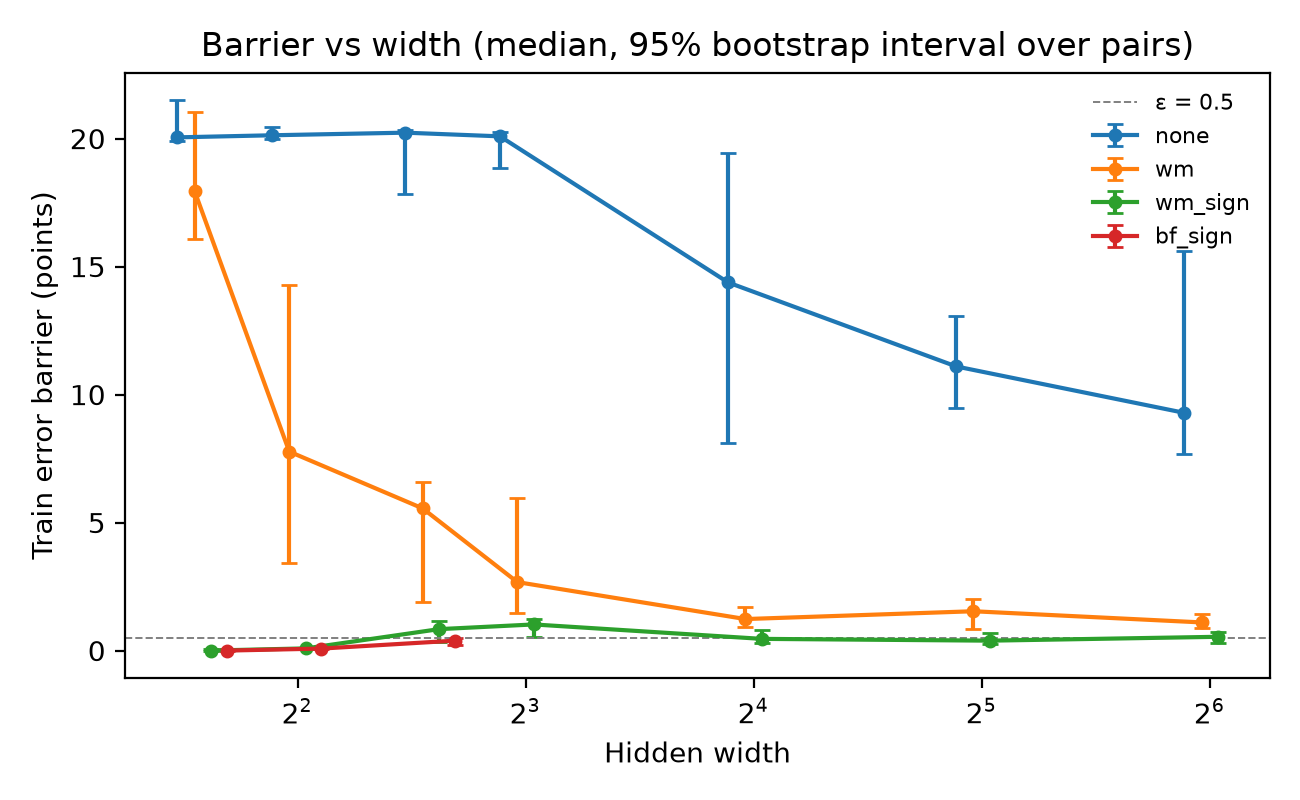
\includegraphics[width=0.82\linewidth]{figures/fig2_barrier_ci.png}
\caption{Study~1 (coffee task). Training-error barrier against hidden width: median over independent pairs, with 95\% bootstrap intervals (10{,}000 resamples of pairs). \md{none}: no alignment. \md{wm}: weight matching over permutations. \md{wm\_sign}: weight matching over permutations and sign flips. \md{bf\_sign}: brute force over all permutations and flips (widths 3--6), chosen by midpoint loss. Dashed line: $\eps = 0.5$ points. Width~3: 11 pairs; widths 4--64: 20 pairs; no width-2 network met the inclusion rule.}
\label{fig:barrier}
\end{figure}

\section{Background and related work}
\label{sec:background}

\paragraph{Barriers.} For networks with parameters $\theta_A, \theta_B$ and a loss or error $L$, the barrier along the straight line is~\cite[Eq.~1]{entezari2022role}
\begin{equation}
B(\theta_A, \theta_B) = \sup_{\alpha \in [0,1]} \Big[ L\big((1-\alpha)\theta_A + \alpha\theta_B\big) - \big((1-\alpha) L(\theta_A) + \alpha L(\theta_B)\big) \Big],
\label{eq:barrier}
\end{equation}
so that $\alpha = 0$ is network $A$. Entezari et al.\ report it at $\alpha = 1/2$ as a surrogate for the supremum~\cite[footnote~3]{entezari2022role}. I evaluate it on a grid of 25 values of $\alpha$ and use the training \emph{error} as $L$ for all verdicts (Section~\ref{sec:setup}).

\paragraph{Symmetries of one-hidden-layer sigmoid networks.} Write the network as
\begin{equation}
f(x) = \sum_{i=1}^{h} s_i\, \sigma(w_i^\top x + b_i) + c, \qquad \sigma(z) = \frac{1}{1+e^{-z}},
\label{eq:net}
\end{equation}
with input weights $w_i$, biases $b_i$, output weights $s_i$ and output bias $c$. Permuting the units leaves $f$ unchanged~\cite{hechtnielsen1990algebraic}. Because $\sigma(-z) = 1-\sigma(z)$, so does a \emph{sign flip} of unit $i$:
\begin{equation}
(w_i, b_i, s_i, c) \;\mapsto\; (-w_i, -b_i, -s_i, c + s_i), \qquad\text{since}\qquad -s_i\sigma(-z) + c + s_i = s_i\sigma(z) + c .
\label{eq:flip}
\end{equation}
This group of permutations and sign flips was described for $\tanh$ networks by Chen et al.~\cite{chen1993geometry}. Sussmann proved that for irreducible one-hidden-layer $\tanh$ networks these are the only symmetries~\cite{sussmann1992uniqueness}, and Kůrková and Kainen characterize functional equivalence for one-hidden-layer networks with more general activation functions~\cite{kurkova1994functionally}; Vla\v{c}i\'c and B\"olcskei restate the lemma behind it, on the symmetries of $\tanh$ itself, as their Lemma~2 and study identifiability for broader classes of activations~\cite{vlacic2020affine}. For sigmoid and $\tanh$, Martinelli et al.~\cite{martinelli2024expand} show that a neuron's input weights are identifiable from the network's function only up to sign. Their Section~4 groups both as ``odd (+ constant)'' activations, for which a unit can be replaced by one with flipped signs, the constant being absorbed by the next layer's bias (Appendix~A.2.2; their classification in Appendix~A.2.3 lists $\tanh$ as odd and the sigmoid as odd plus constant); Theiss et al.\ refine this classification and call such activations constant-odd~\cite[Appendix~B.3]{theiss2026parameter}. Since $\sigma(z) = \tfrac12\big(1+\tanh(z/2)\big)$, a sigmoid network with an output bias is a $\tanh$ network with rescaled weights, so the same holds for Eq.~\eqref{eq:net}. A network is irreducible when no output weight is zero, no unit has zero input weights, and no two units have equal or opposite input parameters $(w_i, b_i)$~\cite{sussmann1992uniqueness} (the last condition is Lemma~1 of~\cite{vlacic2020affine}); in practice I also flag units that are nearly constant on the data. Two limits matter here. First, uniqueness holds for the function on all of $\mathbb{R}^2$; on a finite data set, the set of equivalent networks can only be larger~\cite[Section~I-A]{vlacic2020affine}. Bürgin et al.~\cite{burgin2026beyond} study exactly such approximate, data-dependent symmetries and their effect on linear mode connectivity. Second, if a network is \emph{nearly} reducible, for example because two units almost coincide, it has continuous near-symmetries that no finite search covers.

\paragraph{Related work.} Entezari et al.\ ran a brute-force permutation search on small ReLU networks trained on MNIST~\cite[Appendix~E.3]{entezari2022role}, and Ainsworth et al.\ exhaustively searched the permutations of a hand-built two-hidden-layer ReLU network on a two-dimensional task to show that some solutions admit no linearly connecting permutation~\cite[Appendix~A.6]{ainsworth2023git}. ReLU networks have no sign-flip symmetry, so flips do not arise in either setting. Jordan et al.\ trace much of the barrier that remains after permutation alignment to a collapse in the variance of the interpolated network's activations, and reduce it by renormalizing them (REPAIR)~\cite{jordan2023repair}. Midpoint erasure (Section~\ref{sec:flips}) is an extreme form of this collapse that no renormalization can undo: at $\alpha = \tfrac12$ the erased unit's pre-activation and output weight are both exactly zero. Martinelli et al.\ already use the sign flip to align independently trained networks: before clustering the neurons of several student networks, they ``arbitrarily align all input weight vectors to have a positive $n^{\text{th}}$ element''~\cite[Section~5]{martinelli2024expand}. Pittorino et al.\ removed sign-reversal symmetries together with permutations when aligning independently trained networks with sign activations: they match absolute cosine similarities, apply the permutation, and then flip each unit if that increases the similarity, and they find that removing symmetries lowers the barriers~\cite[Section~3.1.2, Section~4.2 and Fig.~19]{pittorino2022deep}; their networks were wide and binarized, the matching heuristic, and the permutation and sign contributions were not separated. Wiese et al.\ likewise remove $\tanh$ sign flips and then permutations from Markov chain Monte Carlo samples of Bayesian networks, one of which has a single hidden layer of three $\tanh$ units~\cite[Section~5.3 and Appendix~B]{wiese2023towards}. Boufalis et al.~\cite[Appendix~A, Proposition~1]{boufalis2025symmetry} extended weight matching to sign flips for sine and $\tanh$ networks, essentially the \md{wm\_sign} mode used here. They used this sign-aware matcher, exact for one hidden layer and an approximation in deeper networks, only on networks constructed to be equivalent: transformed copies of one sine network with small perturbations (their Section~5.1); in their Appendix~A they note that it can flip signs unnecessarily. On independently trained $\tanh$ CNNs, their Git Re-Basin baseline was permutation-only. Their sign-aware method there was a learned ScaleGMN autoencoder whose decoded networks approximate the originals (their Table~2), so its aligned endpoints are not exact symmetry copies. In a different model class, Kanoh and Sugiyama showed that, for soft decision-tree ensembles, linear mode connectivity requires accounting for tree-specific invariances beyond permutations: a ``subtree flip invariance'', which rests on the same identity $\sigma(-c) = 1-\sigma(c)$, and a splitting-order invariance; they ``performed an exhaustive search to explore all patterns'' of these invariances~\cite[Sections~3.1--3.2]{kanoh2025linear}. Building on these works, I apply exact sign-aware matching to independently trained networks and certify it with an exhaustive search over the complete group. Şimşek et al.~\cite{simsek2021geometry} assumed that at minimal width the global minima are isolated permutation copies, and showed that one extra neuron connects them through straight segments (their Theorem~3.1 and Corollary~4.1); for sigmoid, they remark, about their related Theorem~4.2, that ``the analysis must include additional invariances'' (Remark~4.1). Appendix~\ref{sec:spare} builds on their construction by adding a sign-flip move. Zhan et al.~\cite{zhan2025analyzing} analyze a two-layer ReLU teacher--student model with fixed output weights, no biases and a population loss; from their characterization of the global minima (Lemma~2, from~\cite{lin2024exploring}) they note that when student and teacher widths are equal, any two minima coincide up to permutation, so the permuted barrier is zero (their Figure~4 caption). The width-3 result of Study~1 can be read as an empirical sigmoid analogue, in which the coincidence holds only up to permutations \emph{and} sign flips. Zhao et al.~\cite{zhao2025understanding} relate the connected components of the set of minima to the topology of the symmetry group, build constant-loss curves from continuous symmetries (their Section~6.1), and note that characterizing the minima of nonlinear networks ``requires identifying the complete set of symmetries'' (Section~7). For irreducible one-hidden-layer sigmoid networks that complete set of exact symmetries is known, and this study searches all of it. Ito et al.~\cite{ito2026permutations} show that very wide image networks become linearly connected without any permutation after temperature calibration; I return to their work in Section~\ref{sec:pitfalls}.

\section{Setup and pre-registration}
\label{sec:setup}

\paragraph{Task and data.} The task is the ``coffee roasting'' problem from the Machine Learning Specialization~\cite{ng2022mls}: two features (temperature 150--285\,$^\circ$C, duration 11.5--15.5\,min), and a roast is good inside a triangle bounded by $t > 175$, $d > 12$ and $d \le -\tfrac{3}{85}t + 21$. The data generator is a re-implementation written for this study; it uses the same labeling rule as the course's \texttt{load\_coffee\_data}, checked against a publicly available, unofficial copy of the lab file, since the official copy was not accessible to me; no course files are redistributed with this work. Unlike the lab, which uses 200 points, I draw 2{,}000 fresh training points and 2{,}000 test points (seeds 0 and~1); 20.95\% of the training points are good roasts. Features are standardized with the training statistics. The good region has exactly three edges, so three hidden units are the natural minimum.

\paragraph{Networks and training.} Networks follow Eq.~\eqref{eq:net} with a sigmoid output and binary cross-entropy. I trained widths 2, 3, 4, 6, 8, 16, 32 and 64, with 40 seeds each, using Glorot-uniform weights and zero biases~\cite{glorot2010understanding} and full-batch Adam~\cite{kingma2015adam} (learning rate 0.01, 3{,}000 steps, no weight decay). Because training is full batch, the initialization is the only source of randomness. Before the main run I checked the learning rate against a rule fixed in advance (loss always finite; no rebound of more than 10\% after step 200; final loss within 5\% of the lowest); all 10 check runs (5 seeds at widths 3 and 64) passed.

\paragraph{Inclusion and pairing.} A network is included if its training error is at most 2\%. Included networks are paired disjointly in seed order, so pairs are independent samples. Inclusion was 0 of 40 at width~2, 23 of 40 at width~3 (11 pairs) and 40 of 40 at every larger width (20 pairs). Throughout, ``minimal width'' is meant operationally: width~3 is the smallest tested width at which networks met the inclusion rule under this training protocol. The three triangle edges motivate this choice but do not prove a lower bound; a width-2 sigmoid network that classifies the task is not ruled out.

\paragraph{Barrier.} I evaluate Eq.~\eqref{eq:barrier} at 25 evenly spaced values of $\alpha$. The \emph{training-error barrier}, in percentage points (1 point = 20 of 2{,}000 training examples), decides every verdict, with $\eps = 0.5$ points (10 training examples) as the threshold for ``removed''. The test-error barrier is reported alongside. In Study~1, loss barriers are reported only after output-scale calibration (Section~\ref{sec:pitfalls}); Study~2 reports raw and calibrated loss barriers side by side. Study~1 calibrates over 41 output scales (0.25 to 8) and Study~2 over 81 (0.01 to 16); the range was widened because the Study~1 range proved too narrow for unaligned pairs, and no aligned pair, the pairs every Study~2 hypothesis compares, reached the edge of the Study~2 range (Section~\ref{sec:robust}).

\paragraph{Alignment modes.} Before interpolating, network $B$ is aligned to network $A$ in one of five ways:
\begin{itemize}[leftmargin=*]
\item \md{none}: no alignment.
\item \md{wm}: weight matching~\cite{ainsworth2023git}. For one hidden layer this is a single linear assignment problem: I represent each unit by $u_i = (w_i, b_i, s_i) \in \mathbb{R}^4$ and choose the permutation maximizing $\sum_i u_i^{A\top} u_{\pi(i)}^{B}$ (Hungarian algorithm~\cite{kuhn1955hungarian}).
\item \md{wm\_sign}: the same with sign flips allowed, solved by maximizing $\sum_i |u_i^{A\top} u_{\pi(i)}^{B}|$ and flipping unit $\pi(i)$ by Eq.~\eqref{eq:flip} when its inner product is negative, as in~\cite[Section~3.1.2]{pittorino2022deep} and~\cite[Proposition~1]{boufalis2025symmetry}. The output-bias shift of a flip is not part of the matching objective.
\item \md{bf\_perm} and \md{bf\_sign}: brute force over all permutations (widths up to 8) or all permutations and flips (widths up to 6), choosing the alignment with the lowest loss at the midpoint, the surrogate of~\cite{entezari2022role}.
\end{itemize}
Two further modes, \md{exact\_perm} and \md{exact\_sign}, choose by the full 25-point error barrier instead; these belong to the post-hoc analysis of Section~\ref{sec:b1}.

\paragraph{Pre-registration.} The hypotheses and questions in Table~\ref{tab:prereg} were fixed on 4--5 October 2026 and recorded in a dated research notebook before any network was trained. The numerical thresholds (inclusion rule, line-matching tolerances, $\eps$, the H2 band, and the H1b distance and test) were dated 7--8 October, before the main run on 9 October. The value predicted by H2 reflected the expectation, from Entezari et al.~\cite{entezari2022role} and Ainsworth et al.~\cite{ainsworth2023git}, that networks which learn the same features become linearly connected once their hidden units are matched by a permutation. Three things were \emph{not} dated in advance: the pass fractions named in the falsifiers of Q1, Q3 and Q4, and which aligned mode Q2 should use. None of the answers below depends on them except Q3, which I therefore report as counts only, and Q2, which I therefore report for both aligned modes. This pre-registration was private: its record is the dated notebook, available on request, not a public registry such as OSF, and there is no pre-registration commit because the project was not yet under version control. Everything decided after seeing results is labelled \emph{post-hoc} below. The Study~1 rules are now public in the repository (\texttt{preregistration/v1\_rules\_2026-10.md}); their dates come from the notebook and are not independently timestamped. The Study~2 rules were committed to the public repository before any Study~2 network was trained (Section~\ref{sec:v2}).

\begin{table}[t]
\centering
\small
\caption{Pre-registered hypotheses (H) and questions (Q). A line ``matches'' if its angle differs by at most $10^\circ$ and its offset by at most 0.25 standardized units.}
\label{tab:prereg}
\begin{tabularx}{\linewidth}{@{}lXX@{}}
\toprule
 & Prediction or question & Falsified if \\
\midrule
H1 & More than half of converged width-3 pairs learn the same three lines & Half or fewer of the pairs match on every line \\
H1b & Seeds with higher training error have lines further from the other seeds' & Spearman $\rho \le 0$ over all 40 width-3 seeds \\
H2 & The \md{wm}-aligned blend at width~3 is slightly worse, about 1.8 points & The median falls outside 0.5--3 points \\
H3 & The aligned (\md{wm}) barrier shrinks with width & Width 64's median is not below width 3's (a rise-then-fall counts as a partial miss) \\
\midrule
Q1 & Do independently trained width-3 networks learn the same lines? & --- \\
Q2 & How does the barrier change with width? & --- \\
Q3 & Does weight matching find the barrier-minimizing alignment? & --- \\
Q4 & Do sign flips lower the barrier beyond permutations? & --- \\
\bottomrule
\end{tabularx}
\end{table}

\section{Results}
\label{sec:results}

All values are medians over pairs with 95\% percentile bootstrap intervals~\cite{efron1979bootstrap} (10{,}000 resamples of pairs); with few pairs these intervals are order statistics (for 11 pairs, the 3rd and 9th smallest values, an interval with exact coverage 93.5\%); paired differences are medians of per-pair differences. Appendix~\ref{app:tables} lists every value.

\subsection{Width-3 networks learn the same three lines (H1 supported, H1b supported)}

All 11 of 11 width-3 pairs matched on every line (largest angle difference $2.0^\circ$, largest offset 0.12 standardized units; Figure~\ref{fig:lines}), so H1 is supported and the answer to Q1 is yes. For comparison, 16 of 20 width-4 pairs matched. The claim covers networks that finished training: at a looser 5\% inclusion rule, 10 of 12 width-3 pairs matched, and the two that did not match differed by $39.5^\circ$ and $23.9^\circ$.

For H1b, the Spearman rank correlation~\cite{spearman1904proof} between a seed's training error and its median distance to the other seeds' lines (in \emph{threshold units}: for the worst-matched line, the larger of its angle difference divided by $10^\circ$ and its offset difference divided by 0.25, so that 1 is the edge of the H1 tolerance) is $\rho = 0.800$ [0.625, 0.886] over all 40 width-3 seeds, so H1b is supported. The support comes from two separate groups rather than a smooth trend: 23 seeds that finished training (error 0.65--1.3\%, distance 0.20--0.52 threshold units) and 17 that did not (error 3.65--16.85\%, distance 2.4--10.8). Within each group the correlation is weak to moderate ($\rho = 0.17$ and $0.42$).

\begin{figure}[t]
\centering
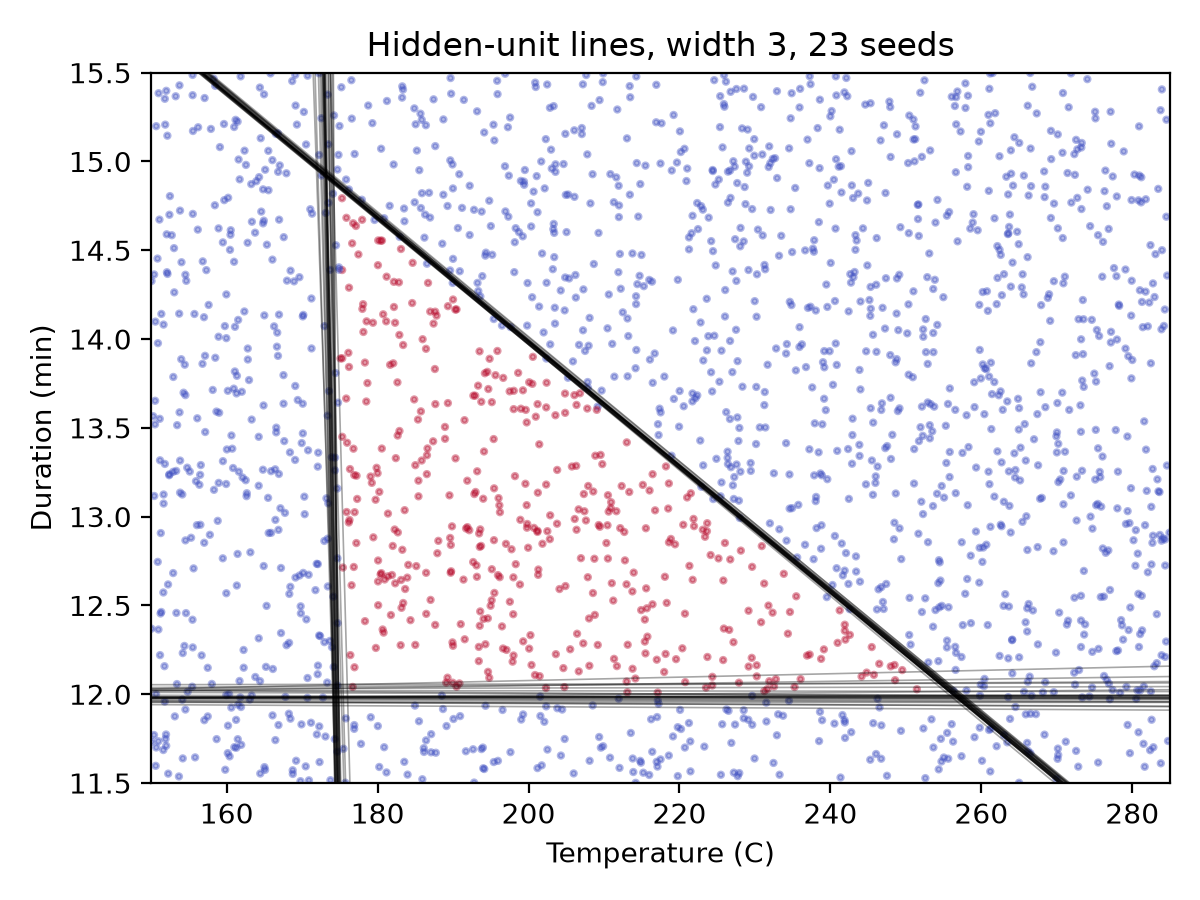
\includegraphics[width=0.62\linewidth]{figures/fig1_lines.png}
\caption{The three hidden-unit lines of all 23 included width-3 networks, drawn in original units over the training data (red: good roasts). Independently trained networks learn the same three edges of the triangle.}
\label{fig:lines}
\end{figure}

\subsection{Permutations leave the barrier; sign flips remove it (H2 not supported, Q4 yes)}
\label{sec:flips}

Although the width-3 networks compute the same three lines, the median \md{wm} barrier is \textbf{17.95 [16.07, 21.05] points}, far outside the pre-registered 0.5--3 band, so H2 is not supported. In hindsight H2 was mis-specified: its rationale (matched features connect once permuted) predicts a barrier near zero, which also lies outside the band, and pairs that needed no flip did have \md{wm} barriers near zero (0.01 points in Study~1; medians 0.02--0.07 in Study~2; post-hoc). H2's failure is therefore not itself evidence for sign flips; that evidence is Q4 and, in Study~2, H4b. Without alignment the median is 20.05 points. Reordering hidden units alone does not align these networks.

Allowing sign flips changes the picture (Figures~\ref{fig:barrier} and~\ref{fig:paths}). The pre-registered Q4 measure compares the best permutation (\md{bf\_perm}) with the best permutation and flip pattern (\md{bf\_sign}): flips lowered the training-error barrier by more than $\eps$ in \textbf{10 of 11} pairs at width~3, 16 of 20 at width~4 and 16 of 20 at width~6, with median drops of 17.79, 7.72 and 3.37 points (paired interval at width~3: $-17.79$ [$-20.18$, $-15.14$]). The best sign-aware alignment used at least one flip in 10 of 11 width-3 pairs. Descriptively (post-hoc), 0, 1, 2 and 3 units were flipped in 1, 5, 4 and 1 pairs; these counts are close to those expected if each unit's relative orientation were a fair coin (1.4, 4.1, 4.1 and 1.4 of the 11 pairs), but Study~2 rules out that reading (post-hoc): no pair at $h^* = 4$ needed three or four flips, against about 5--8 and 1--2 expected per task under fair coins, and only one width-3 pair of 83 needed three flips, against 10.4 expected. Orientations are therefore biased towards agreement; the cause of the bias is not studied here. The \md{wm\_sign} barrier at width~3 is 0.00 [0.00, 0.05]. Beyond the Q4 measure, the per-pair difference \md{wm\_sign}~$-$~\md{wm} has its whole interval below zero at every width, from $-17.84$ [$-21.05$, $-16.07$] at width~3 to $-0.61$ [$-0.93$, $-0.38$] at width~64.

The mechanism is visible in Eq.~\eqref{eq:flip}. Two networks that differ by a flip of unit $i$ compute the same function, but halfway along the straight line between them that unit's input weights, bias and output weight all blend to zero. Its contribution to the logit then changes by $-s_i(\sigma(z) - \tfrac12)$, which is up to $|s_i|/2$ in size. On one trained width-3 network (seed~1, unit~2, $s = -11.14$), the straight blend to its own flipped copy changes the logit by up to 5.57 and reaches 20.95\% training error (Figure~\ref{fig:spare}). Permutation matching cannot undo such a flip; it can only choose which unit is paired with which.

\begin{figure}[t]
\centering
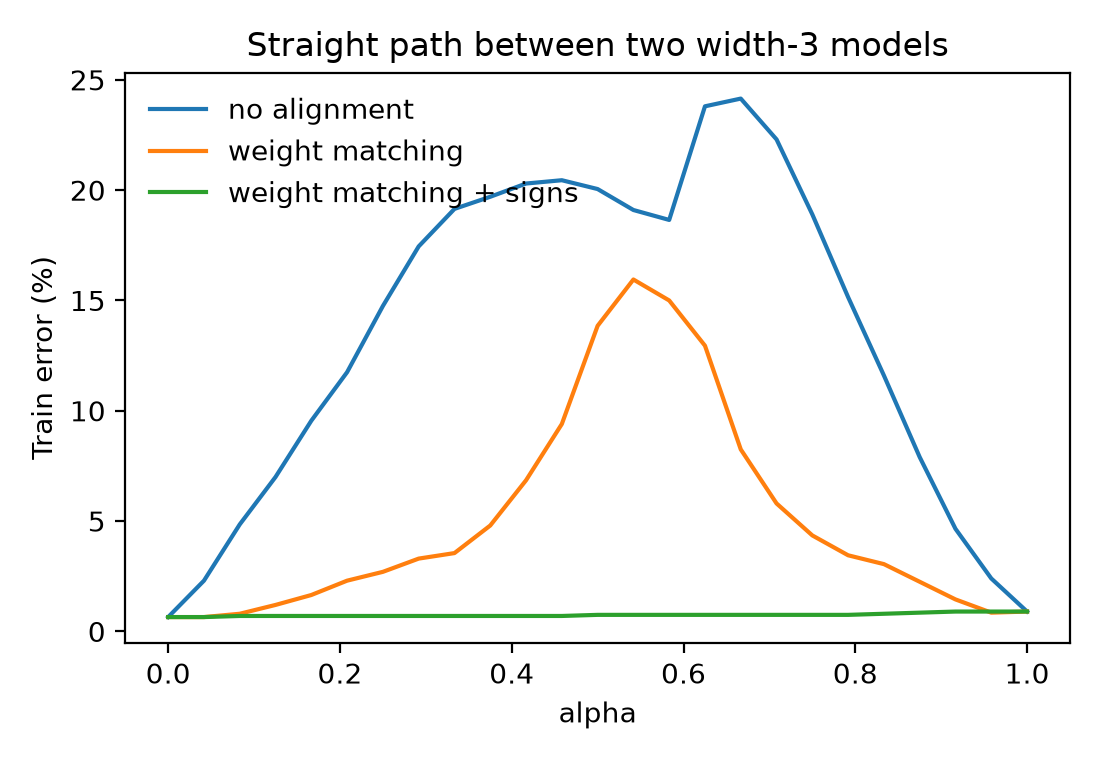
\includegraphics[width=0.6\linewidth]{figures/fig3_paths.png}
\caption{Training error along the straight path between the first pair of width-3 networks ($\alpha = 0$: network $A$), with no alignment, with weight matching, and with weight matching plus sign flips.}
\label{fig:paths}
\end{figure}

\subsection{Post-hoc: an exhaustive search over the complete group}
\label{sec:b1}

This post-hoc analysis asks how large a barrier remains after searching \emph{every} permutation and sign flip and choosing by the full 25-point error barrier rather than the midpoint. The search is exhaustive over the transformations; the barrier itself is evaluated on this grid of 25 interpolation weights, so it is a lower bound on the maximum over the continuous segment. The rules for this analysis, including the irreducibility checks and the threshold for ``removed'' (upper quartile at most $\eps$), were dated on 9 October, before the search ran. A network was flagged \emph{nearly reducible} if its smallest output weight was below 5\% of its largest, if two of its own units matched under the same line tolerance used for H1, or if a unit's activation varied by less than 0.01 (standard deviation) over the training data.

\begin{table}[t]
\centering
\small
\caption{Post-hoc complete-group search (\md{exact\_sign}): training-error barrier left after the best of all $2^h h!$ permutation-and-flip combinations, chosen by the full barrier.}
\label{tab:b1}
\begin{tabular}{@{}rrcrr@{}}
\toprule
Width & Pairs & Residual: median / upper quartile / max & Pairs above $\eps$ & Pairs with a nearly reducible network \\
\midrule
3 & 11 & 0.00 / 0.04 / 0.11 & 0 & 0 of 11 \\
4 & 20 & 0.08 / 0.11 / 1.44 & 1 & 20 of 20 \\
6 & 20 & 0.33 / 0.52 / 1.78 & 5 & 20 of 20 \\
\bottomrule
\end{tabular}
\end{table}

At width~3, the residual is at most \textbf{0.11 points} in all 11 pairs (Table~\ref{tab:b1}). Every included width-3 network is irreducible: the closest pair of units within a network is at a median of 4.2 threshold units, where 1 would mean the same line. The search therefore covers every exact symmetry these networks have, and exact symmetries account for essentially the whole barrier. This does not show that the two networks of a pair compute the same function: identifiability fixes the symmetries available to each network, and the small residual shows only that the best of them brings the pair close. The result holds at 1\% and 5\% inclusion (maximum residual 0.09 and 0.47 points; no included network nearly reducible).

At widths 4, 6 and 8, nearly every network has two units on almost the same line, with a spare unit copying one of the three lines the task needs (37 of 40 networks at width~4, 38 of 40 flagged by any rule, and all networks at widths 6 and~8). Such networks may have near-symmetries outside the finite group, exact or holding only on the data, so their residuals are upper bounds only, a risk recorded before the search. Width~6 falls short of the ``removed'' threshold by 0.02 (upper quartile 0.517). I decided after seeing the width-6 result not to run the signed search at width~8 (10.3 million candidates per pair), since its networks are all nearly reducible.

For the question raised by Ainsworth et al.~\cite[Section~5.3]{ainsworth2023git}, the answer \emph{for these sigmoid networks on this task} is \emph{another symmetry}: permutation matching leaves a large barrier because a sign flip is not a permutation, and once flips are included, both weight matching and the exhaustive search remove the barrier at width~3. A sign flip is an affine relation between activations, since the flipped unit outputs $1-\sigma(z)$; this fits their own hypothesis that ``linear, possibly non-permutation, relationships connect the layer-wise activations between models trained by SGD''~\cite[Section~7]{ainsworth2023git}. ReLU networks have no sign-flip symmetry, so this explanation does not carry over to the ReLU networks of their experiments, where the question remains open.

\subsection{Width dependence (H3's endpoint prediction supported, Q2)}

The median \md{wm} barrier falls from 17.95 points at width~3 to \textbf{1.10 [0.86, 1.42]} at width~64, so H3's endpoint prediction is supported. The observed trend is broadly decreasing but not monotonic: the median rises by 0.31 points between width~16 (1.23) and width~32 (1.54), below $\eps$, with overlapping intervals ([0.91, 1.68] and [0.83, 2.03]). The pre-registered falsifier did not say how to treat a small rise after a long fall, so I report the non-monotonicity rather than classify it.

For Q2: without alignment the median barrier stays near 20 points up to width~8 and then falls to 9.29 [7.67, 15.60] at width~64. With \md{wm} it shrinks, but its upper quartile stays above $\eps$ at every width (1.61--20.31). With \md{wm\_sign} the barrier is removed at widths 3 and~4 (upper quartiles 0.04 and 0.11), but not from width 6 to~64 (upper quartiles 0.77--1.30, medians 0.39--1.02). Because Q2 did not name an aligned mode, both are reported (post-hoc; Section~\ref{sec:setup}). The test-set barrier gives the same answers at every width.

\subsection{Does weight matching find the best alignment? (Q3, counts only)}

Table~\ref{tab:q3} compares weight matching with brute force, counting a pair as ``same'' when the two barriers differ by at most $\eps$. Under the pre-registered comparison, weight matching ``beat'' brute force in 7 pairs, by up to 20 points. This is possible only because brute force chose by the midpoint. Entezari et al.\ found the midpoint an accurate surrogate in their settings~\cite[footnote~3]{entezari2022role}, but in these small networks the error peak sometimes lies elsewhere: in all 7 pairs it lay more than 0.05 from $\alpha = 0.5$ ($\alpha = 0.375$ to $0.708$). The post-hoc exact search removes this artifact. With sign flips, weight matching finds the best alignment at widths 3 and~4 and drifts from it as width grows. With flips, the midpoint and full-barrier rules never differed by more than $\eps$.

\begin{table}[t]
\centering
\small
\caption{Q3: weight matching against brute force (pairs where weight matching is the same / worse / better, within $\eps$). Left: pre-registered comparison with midpoint-chosen brute force. Right: post-hoc comparison with the exact search. ---: not computed; the signed search was not run at width~8 (10.3 million candidates per pair; see Section~\ref{sec:b1}).}
\label{tab:q3}
\begin{tabular}{@{}rcc|cc@{}}
\toprule
 & \multicolumn{2}{c|}{Pre-registered (midpoint)} & \multicolumn{2}{c}{Post-hoc (exact)} \\
Width & \md{wm} vs.\ \md{bf\_perm} & \md{wm\_sign} vs.\ \md{bf\_sign} & \md{wm} vs.\ \md{exact\_perm} & \md{wm\_sign} vs.\ \md{exact\_sign} \\
\midrule
3 & 8 / 2 / 1 & 11 / 0 / 0 & 7 / 4 / 0 & 11 / 0 / 0 \\
4 & 11 / 4 / 5 & 19 / 1 / 0 & 15 / 5 / 0 & 19 / 1 / 0 \\
6 & 14 / 6 / 0 & 11 / 9 / 0 & 12 / 8 / 0 & 11 / 9 / 0 \\
8 & 9 / 10 / 1 & --- & 8 / 12 / 0 & --- \\
\bottomrule
\end{tabular}
\end{table}

\section{Study 2: five tasks and their minimal widths (pre-registered)}
\label{sec:v2}

Study~1 (Sections~\ref{sec:setup}--\ref{sec:results}) rests on one task, one width and 11 pairs, with the decisive search chosen after the main run. Study~2 asks whether its result holds on new tasks, at their own minimal widths, with more pairs, under rules fixed in public beforehand.

\paragraph{Pre-registration and firewall.} The Study~2 rules (\texttt{preregistration/v2\_rules.md}) were committed to the public repository (commit \texttt{349aa3a}, 19 October 2026) before any Study~2 network was trained. Training (Stage~1) used training error only; its outputs were then frozen with a SHA-256 fingerprint of every model file (commit \texttt{4c07b33}), and the analysis code refuses to run on changed files. Clarifications and deviations are logged with dates in \texttt{preregistration/DEVIATIONS.md} (D1--D13). D7 was written after the training counts and before any barrier, and D8, D9 and D12 after all results; all four are marked below. D10 and D11 record text corrections that changed no result. The rules also fix the title in advance: the present title if H4a holds on every analysable task (the coffee task and at least three polygons), ``\dots\ in Small Sigmoid Networks'' if it holds on some, and ``\dots\ in Width-3 Sigmoid Networks'' if only on the coffee task.

\paragraph{Tasks.} T0 is the coffee task of Study~1, with 80 new seeds added at width~3 (120 in total). T3--T6 are convex polygons with $k = 3, 4, 5, 6$ edges, drawn once by a fixed rule: irregular, off-centre, area 21\% of the square $[-1,1]^2$ to match the coffee task's positive rate, every interior angle at most $165^\circ$ and every edge at least 0.25 long. Inputs are uniform on the square (2{,}000 training and 2{,}000 test points); labels are exact, so the data are separable. Model, initialization, optimizer, inclusion rule (2\%), pairing and barrier are exactly as in Study~1. Each polygon task trains 100 seeds at widths $k-2$ to $k+2$ (at least 2). The original 40 coffee seeds were retrained to record their error 300 steps before the end. Their first 11 pairs reproduce Study~1's residuals exactly (0.03, 0, 0, 0.05, 0, 0.08, 0.11, 0.01, 0, 0, 0 points). The coffee task's 36 pairs therefore include Study~1's 11, so T0 is a re-test on an enlarged sample, not an independent replication; on the 24 pairs made only of new seeds (40--119) the residual is median 0.03, upper quartile 0.05, maximum 0.17 points. The four polygon tasks are new.

\paragraph{Minimal width is measured, not assumed.} $h^*$ is the smallest width at which at least 10 networks met the inclusion rule. At 2\% it is 3 for both triangles and 4 for the quadrilateral, the pentagon \emph{and} the hexagon. At 1\% it equals $k$ for every polygon. The width grid starts at $k-2$, so for the hexagon at 2\% (and the hexagon and pentagon at 5\%) $h^*$ is the smallest width trained and is an upper bound, not a measurement. Four sigmoid units can draw four lines that cut off the small corners of a pentagon or hexagon and still misclassify fewer than 40 of 2{,}000 points. ``Minimal width'' is therefore tied to an error tolerance, and I report both.

\paragraph{Analysis.} At $h^*$, every disjoint pair of included networks was aligned by \md{none}, \md{wm}, \md{wm\_sign}, and by exhaustive search over all permutations (\md{exact\_perm}) and all permutations and flips (\md{exact\_sign}), each chosen by its 25-point training-error barrier (the Study~1 rule). A \emph{flip pair} is a pair whose \md{exact\_sign} alignment flips at least one unit; this definition is fixed in the rules and does not depend on the size of any barrier. Each alignment was scored by four measures: training-error barrier (deciding), test-error barrier, raw loss barrier, and loss barrier calibrated over 81 output scales from 0.01 to 16. The pre-registered hypotheses are:
\begin{itemize}[leftmargin=*]
\item \textbf{H1}: all pairs learn the same lines.
\item \textbf{H4a}: the \md{exact\_sign} residual has an upper quartile $\le \eps$.
\item \textbf{H4b}: in flip pairs, \md{exact\_perm} leaves a median above 2 points.
\item \textbf{H4c}: \md{wm\_sign} is within $\eps$ of \md{exact\_sign} in at least 80\% of pairs.
\item \textbf{H5}: \md{exact\_perm} $>$ \md{exact\_sign} in at least 90\% of flip pairs under each of the four measures.
\item \textbf{H7}: the weights predict the size of the barrier (Section~\ref{sec:v2h7}).
\end{itemize}
Each threshold's justification is in the rules file. Inclusion counts per width, flip counts and results above $h^*$ are in Appendix~\ref{app:v2more}.

\begin{table}[t]
\centering\small
\caption{Study~2 main analysis (2\% inclusion), at the measured minimal width $h^*$. Residual: \md{exact\_sign} training-error barrier, median / upper quartile / maximum, in points. Perm-only: median \md{exact\_perm} barrier in pairs that need a flip. H4c: share of pairs where \md{wm\_sign} is within $\eps$ of \md{exact\_sign}. H5: smallest share, over the four measures, of flip pairs where \md{exact\_perm} $>$ \md{exact\_sign}. Every network was irreducible (no pair flagged). Generated from \texttt{results\_v2/}.}
\label{tab:v2}
\begin{tabular}{@{}lcccccccc@{}}
\toprule
Task & $h^*$ & Pairs & Same lines & Residual & Perm-only & Flip pairs & H4c & H5 \\
\midrule
Coffee (triangle) & 3 & 36 & 36/36 & 0.02 / 0.05 / 0.17 & 19.98 & 32 & 100\% & 100\% \\
Triangle & 3 & 47 & 47/47 & 0.03 / 0.06 / 0.13 & 21.65 & 36 & 100\% & 100\% \\
Quadrilateral & 4 & 32 & 30/32 & 0.04 / 0.07 / 9.58 & 17.53 & 26 & 97\% & 96\% \\
Pentagon & 4 & 21 & 21/21 & 0.05 / 0.07 / 0.15 & 12.38 & 14 & 100\% & 100\% \\
Hexagon & 4 & 29 & 23/29 & 0.06 / 0.13 / 4.81 & 9.95 & 21 & 97\% & 100\% \\
\bottomrule
\end{tabular}
\end{table}

\subsection{Pre-registered verdicts}
\label{sec:v2verdicts}

H4a, H4b, H4c and H5 hold for all five tasks (Table~\ref{tab:v2}). Allowing sign flips turns a median barrier of 9.95--21.65 points into an upper-quartile residual of at most 0.13 points. In 129 of 165 pairs the best alignment needed at least one flip. The ordering holds under every measure, so it is not an artifact of the error metric saturating. Under the training-error barrier the ordering is nearly guaranteed: \md{exact\_sign} minimizes that barrier, on the same grid, over a set of alignments that contains every permutation, so it can fail only through a tie. The informative tests are therefore the test-error, raw-loss and calibrated-loss barriers, which the search did not optimize; the H5 column of Table~\ref{tab:v2} is the smallest share over all four measures. H1 fails for the quadrilateral (2 of 32 pairs) and the hexagon (6 of 29); Section~\ref{sec:v2lines} examines those pairs. For the hexagon this meets item~3 of the pre-registered list of outcomes that would count against the account ($h^* < k$ with H1 failing): four units suffice, and 6 of 29 pairs learn different lines. Item~4 did not occur (14 of 187 excluded networks were classed as wrong minima). Under the pre-registered title rule, these verdicts give the present title. After exact alignment, the networks of a same-line pair remain genuinely different parameter vectors (relative distance 0.04--0.66; median over all pairs 0.23), yet the barrier closes: the symmetry, not proximity, does the work.

\paragraph{Sensitivity (pre-registered at 1\% and 5\%; $h^*$ re-derived by D7).} Table~\ref{tab:v2sens}. At 1\%, $h^* = k$ for every polygon, and the claim holds for every task except the pentagon at width~5. At 5\%, the claim holds for every task except the hexagon at width~4. Under the title rule, each sensitivity run alone would give ``Small Sigmoid Networks''. The title follows the rule at the main 2\% threshold, as pre-registered, and these two failures are part of the result.

\begin{table}[t]
\centering\small
\caption{Inclusion sensitivity. $h^*$ is re-derived at each threshold from training error only (D7). Residual: upper quartile of the \md{exact\_sign} training-error barrier, in points. Pairs and same-line counts exclude pairs with a nearly reducible network (two, for the hexagon at 5\%).}
\label{tab:v2sens}
\begin{tabular}{@{}llccccc@{}}
\toprule
Inclusion & Task & $h^*$ & Pairs & Same lines & Residual (UQ) & H4a \\
\midrule
1\% & Coffee (triangle) & 3 & 28 & 28/28 & 0.04 & yes \\
1\% & Triangle & 3 & 46 & 46/46 & 0.06 & yes \\
1\% & Quadrilateral & 4 & 28 & 28/28 & 0.07 & yes \\
1\% & Pentagon & 5 & 18 & 11/18 & 3.26 & \textbf{no} \\
1\% & Hexagon & 6 & 30 & 22/30 & 0.09 & yes \\
\midrule
2\% & Coffee (triangle) & 3 & 36 & 36/36 & 0.05 & yes \\
2\% & Triangle & 3 & 47 & 47/47 & 0.06 & yes \\
2\% & Quadrilateral & 4 & 32 & 30/32 & 0.07 & yes \\
2\% & Pentagon & 4 & 21 & 21/21 & 0.07 & yes \\
2\% & Hexagon & 4 & 29 & 23/29 & 0.13 & yes \\
\midrule
5\% & Coffee (triangle) & 3 & 38 & 34/38 & 0.05 & yes \\
5\% & Triangle & 3 & 47 & 47/47 & 0.06 & yes \\
5\% & Quadrilateral & 3 & 48 & 44/48 & 0.22 & yes \\
5\% & Pentagon & 3 & 46 & 46/46 & 0.18 & yes \\
5\% & Hexagon & 4 & 48 & 18/48 & 2.58 & \textbf{no} \\
\bottomrule
\end{tabular}
\end{table}

\subsection{Exploratory: learning the same lines suffices}
\label{sec:v2lines}

Splitting the \md{exact\_sign} residual by whether a pair passed the same-line test, a split decided after seeing the results (D9), gives Table~\ref{tab:v2lines}:
\begin{itemize}[leftmargin=*]
\item At 2\%, all 157 same-line pairs end at or below 0.21 points, across all five tasks.
\item The 8 pairs that learned different lines keep 2.38--9.58 points.
\item Both sensitivity failures coincide with many different-line pairs: 7 of 18 pentagon pairs at 1\% and 30 of 48 hexagon pairs at 5\%.
\end{itemize}
The relation is asymmetric. Over the three thresholds, 328 of 331 distinct same-line pairs ended below $\eps$ (maximum 0.74 points). A pair that fails the line test, however, can still be nearly connected when its lines differ only slightly beyond the tolerance: 23 of 58 distinct different-line pairs ended below $\eps$ (median 0.17 points at 1\%). The split therefore also depends on the line tolerance ($10^\circ$, 0.25), which defines H1. Repeating it post hoc with the tolerance halved ($5^\circ$, 0.125) and doubled ($20^\circ$, 0.5) (D12) leaves the first direction intact: all 290 distinct same-line pairs end below $\eps$ at the halved tolerance, and 342 of 345 at the doubled one. The second direction moves with the tolerance: the share of different-line pairs below $\eps$ falls from 61 of 99 (halved) to 23 of 58 (pre-registered) and 9 of 44 (doubled). Pairs whose lines differ only slightly are often still connected; pairs whose lines differ by more than $20^\circ$ or 0.5 units mostly keep a barrier (35 of 44).

This links the empirical result to identifiability: if two irreducible networks compute the same function, Sussmann's theorem~\cite{sussmann1992uniqueness} leaves only permutations and flips, and the question becomes whether trained networks reach the same function. In these data, pairs that learned the same lines were almost always closed by the exact group; pairs whose lines clearly differed kept a barrier (2.38--9.58 points at 2\%).

\begin{table}[t]
\centering\small
\caption{Exploratory (D9): \md{exact\_sign} residual (points) split by the same-line test, pooled over the five tasks. A pair is counted once per threshold, so a pair can appear in more than one row; over the three thresholds there are 331 distinct same-line pairs (3 above $\eps$) and 58 distinct different-line pairs (23 at or below $\eps$).}
\label{tab:v2lines}
\begin{tabular}{@{}lccccccc@{}}
\toprule
& \multicolumn{4}{c}{Same lines} & \multicolumn{3}{c}{Different lines} \\
\cmidrule(lr){2-5}\cmidrule(lr){6-8}
Inclusion & Pairs & Median & Max & $> \eps$ & Pairs & Median & Range \\
\midrule
2\% & 157 & 0.03 & 0.21 & 0 & 8 & 3.74 & 2.38--9.58 \\
1\% & 135 & 0.03 & 0.20 & 0 & 15 & 0.17 & 0.00--4.27 \\
5\% & 189 & 0.06 & 0.74 & 3 & 38 & 1.06 & 0.02--6.06 \\
\bottomrule
\end{tabular}
\end{table}

\subsection{Networks that failed the inclusion rule}

At $h^*$, each network above 2\% training error was classified by a pre-registered rule, first match wins:
\begin{itemize}[leftmargin=*]
\item \textbf{degenerate}: nearly reducible;
\item \textbf{not converged}: its error still changed in the last 300 steps;
\item \textbf{wrong minimum}: some edge of the polygon has no matching unit line.
\end{itemize}
Under this order, 148 of 187 were classed not converged, 14 wrong minima and 25 degenerate (Table~\ref{tab:v2excl}). The classes overlap substantially. 147 of the 148 networks classed not converged also miss a polygon edge, and in 20 of them the error rose rather than fell in the last 300 steps. At $h^* = 4$ for the pentagon and hexagon, every network misses an edge by construction. I therefore do not claim that separate basins are rare. The claim is stated for networks that reach the inclusion threshold. Including every run regardless of inclusion (exploratory) raises the \md{exact\_sign} residual to a median of 0.03--1.22 points by task, as expected for unfinished networks.

\begin{table}[t]
\centering\small
\caption{Classes of networks that failed the 2\% inclusion rule at $h^*$ (pre-registered classification).}
\label{tab:v2excl}
\begin{tabular}{@{}lccccc@{}}
\toprule
Task & Failed inclusion & Not converged & Wrong minimum & Degenerate & Other \\
\midrule
Coffee (triangle) & 48 & 35 & 1 & 12 & 0 \\
Triangle & 6 & 4 & 2 & 0 & 0 \\
Quadrilateral & 35 & 26 & 2 & 7 & 0 \\
Pentagon & 57 & 48 & 5 & 4 & 0 \\
Hexagon & 41 & 35 & 4 & 2 & 0 \\
\bottomrule
\end{tabular}
\end{table}

\subsection{H7: do the weights predict the size of the barrier? (not supported)}
\label{sec:v2h7}

The midpoint-erasure mechanism (Section~\ref{sec:flips}) suggests that the barrier left by the best flip-free permutation should grow with $M = \sum_{i \in F} |s_i|/2$, the bound on the midpoint logit shift summed over the flipped units $F$.

\textbf{Pre-registered test.} Spearman $\rho(M, B_F)$, where $B_F$ is the error barrier with the \md{exact\_sign} permutation applied without its flips, pooled over tasks. Over 129 pairs, $\rho = 0.007$ (95\% bootstrap interval $[-0.18, 0.19]$). The pre-registered rule labels this result ``weak'' because the interval includes zero. Since $\rho$ is indistinguishable from zero, I report H7 as \textbf{not supported}, a more conservative wording than the rule requires. In the sensitivity runs, $\rho = -0.16$ $[-0.35, 0.03]$ at 1\% and $-0.21$ $[-0.37, -0.05]$ at 5\%, neither positive; the loss-based re-test was run at 2\% only.

\textbf{Why it failed (post hoc).} $B_F$ sits near each task's positive rate: median 17--22 points against positive rates of 18.8--22.1\%. Once a substantial unit is erased at the midpoint, the blend predicts ``negative'' almost everywhere. The error barrier saturates at the trivial classifier and cannot grow with $M$. The ordering tests (H5) are immune to this ceiling, but magnitudes are not. Testing H7 on the error barrier was a design error on my part. The same ceiling limits every error-barrier magnitude in this paper, including the Perm-only medians of Table~\ref{tab:v2}: they show that the barrier is large, not how large; orderings within a pair (H5) are unaffected.

\textbf{Exploratory re-test (D8, decided after seeing the result).} Repeating the test on loss barriers, which have no such ceiling, the mechanism does predict magnitude:
\begin{itemize}[leftmargin=*]
\item raw loss: $\rho(M, B_F) = 0.86$ (95\% interval $[0.79, 0.90]$, 129 pairs), positive in every task (0.70--0.94);
\item calibrated loss: $\rho = 0.65$ ($[0.54, 0.75]$), also positive in every task (0.52--0.84).
\end{itemize}
Raw losses grow with the overall weight scale, and so does $M$, so part of the raw correlation may reflect scale. The calibrated loss removes most of the output-scale effect and still gives $\rho = 0.65$. Because this test was chosen after H7 failed, it supports the mechanism only as an exploratory result. A confirmatory test needs a fresh, pre-registered run.

\subsection{Post-hoc: how secure are the verdicts?}
\label{sec:v2posthoc}

These checks were added after all results (D13), use only the released result and model files, and change no verdict.

\paragraph{Uncertainty in the pass rate.} The upper-quartile rule is a point estimate. At $h^*$, the number of pairs whose residual is at most $\eps$, with a one-sided 95\% Clopper--Pearson lower bound on the share of such pairs~\cite{clopper1934use} in brackets, is 36/36 (0.92) for the coffee task, 47/47 (0.94) for the triangle, 30/32 (0.82) for the quadrilateral, 21/21 (0.87) for the pentagon and 23/29 (0.63) for the hexagon. Four tasks pass with a lower bound of at least 0.82. The hexagon's H4a pass (23 of 29 pairs; lower bound 0.63) is not statistically secure: its uncertainty includes failure. Over the five tasks, all 157 same-line pairs end within $\eps$ (lower bound 0.98); every pair that fails learned different lines (Section~\ref{sec:v2lines}). Using every pair of included networks instead of disjoint pairs (with \md{wm\_sign}, which gives the same per-task counts as \md{exact\_sign} on the disjoint pairs), all 11{,}075 same-line pairs end within 0.27 points, and the hexagon passes 1{,}303 of 1{,}711 pairs (76\%).


\paragraph{Choice of $\eps$.} At 2\% inclusion, same-line residuals are at most 0.21 points and different-line residuals at least 2.38. Every H4a verdict, at all three inclusion thresholds, is unchanged for any $\eps$ between 0.23 and 2.57 points, so the value 0.5 does not decide the outcome.

\paragraph{Selection on the reported quantity.} \md{exact\_sign} is chosen by the barrier it reports. \md{wm\_sign}, which never evaluates a barrier, gives the same per-task pass counts at every inclusion threshold. The test-error barrier, which the selection never sees, gives the same counts at 1\% and 2\% inclusion and differs by at most three pairs per task at 5\%. On the test-error barrier, \md{exact\_perm} exceeds \md{exact\_sign} by more than $\eps$ in 128 of 129 flip pairs; in the remaining quadrilateral pair \md{exact\_perm} is lower by 0.45 points.

\paragraph{Selection by the inclusion rule.} For the triangle task the 2\% rule falls in a gap in training error (largest included 1.30\%, next 14.85\%). At $h^* = 4$ it cuts a continuum: 11, 75 and 90 of the 100 quadrilateral, pentagon and hexagon networks end between 1.5\% and 3\%. Within the included networks the residual is not related to the training error of the worse endpoint (Spearman $\rho$ between $-0.43$ and $0.25$ across tasks).

\paragraph{Irreducibility margins.} Over all included networks at $h^*$, the smallest ratio of output weights is 0.46 (flag below 0.05), the closest pair of units within a network is 4.1 threshold units apart (flag below 1), and the smallest activation standard deviation is 0.25 (flag below 0.01). Any reasonable choice of flags certifies the same networks as irreducible.

\section{Measurement pitfalls}
\label{sec:pitfalls}

\paragraph{Training length inflates loss barriers.} The coffee labels are separable, so cross-entropy keeps growing the weights: after 3{,}000 steps the median weight norm (input and output weights of included networks) rises from 32.2 at width~3 to 66.5 at width~64 (Appendix~\ref{app:b4}). A misclassified point's loss grows with the weight scale; for linear predictors, Soudry et al.\ prove that gradient descent on separable data drives the weight norm to infinity, so that the loss on misclassified points keeps increasing (their Lemma~1 and Section~3)~\cite{soudry2018implicit}. Raw loss barriers depend on training length and would mix that into the width trend. Zhao et al.\ make a related point precise: with a rescaling symmetry, two parameter settings of the same function can have an arbitrarily large loss barrier between them~\cite[Proposition~5.3]{zhao2025understanding}. I therefore base every verdict on the error barrier and report loss barriers only after choosing the best of 41 output scales (0.25 to 8, log-spaced) at each blend point, an idea similar in spirit to the temperature calibration of Ito et al.~\cite{ito2026permutations}. This range proved too narrow for 43 of 131 unaligned pairs, whose best scale sat at the lower edge, so calibrated losses for unaligned pairs are only partly calibrated. Aligned pairs almost never hit the edge.

\paragraph{Weight decay.} A side-check with L2 regularization (rule dated before the run) is reported in Appendix~\ref{app:b4}; no network met the inclusion rule, so it gives no verdict and does not bear on the findings of Ito et al.

\section{Robustness}
\label{sec:robust}

\begin{itemize}[leftmargin=*]
\item \textbf{Inclusion threshold (Study~1).} Rerunning the Study~1 analysis at 1\% and 5\% inclusion changes no verdict. (In Study~2, two H4a verdicts change; Section~\ref{sec:v2verdicts}.) Two qualifications: at 1\%, the width-3 paired intervals for the flip effect reach zero at their upper end (\md{wm\_sign}~$-$~\md{wm}: $-17.70$ [$-22.16$, 0.00]), because 3 of 9 pairs needed no flip at all, although the count-based Q4 answer stands; at 5\%, H1 holds with 10 of 12 pairs.
\item \textbf{Test set.} The test-error barrier tracks the training-error barrier at every width (for example, \md{wm} at width~3: 17.95 training, 18.95 test).
\item \textbf{Grid density.} In Study~2 (pre-registered), re-measuring every alignment at $h^*$ on 97- and 385-point grids changes no verdict: the largest change in an \md{exact\_sign} residual is 0.02 points, and calibration never hit the edge of its scale grid for an aligned pair (5 of 165 unaligned pairs did). In Study~1 (post-hoc), re-measuring the width-3 exhaustive-search alignments on nested 97- and 385-point grids moves the maximum residual from 0.11 to 0.12 points (2\% inclusion) and from 0.47 to 0.52 (5\%). The 25-point barrier is a close lower bound.
\item \textbf{Reproduction.} Retraining the original 40 coffee seeds in Study~2 reproduced Study~1's residuals exactly. A clean copy of the project, run from one script on the same machine, reproduced the main result files byte for byte (see the Reproducibility statement).
\end{itemize}

\section{Limitations}
\label{sec:limits}

\begin{itemize}[leftmargin=*]
\item One architecture (one hidden layer, sigmoid), two-dimensional convex-polygon tasks with separable labels, and one optimizer setting (3{,}000 full-batch Adam steps). I did not test $\tanh$ (related by an affine change of parameters), depth or real data.
\item The thin networks of Ainsworth et al.\ are ReLU networks, which have no sign flip; this study answers only the sigmoid analogue of their question.
\item Minimal width is operational and depends on the error tolerance (Section~\ref{sec:v2}); the claim fails for one task at each sensitivity threshold. No hypothesis depends on minimality: the completeness of the search needs irreducibility, which is verified for every analysed network (Section~\ref{sec:v2posthoc}).
\item ``Exact symmetry'' means equality of the function on all inputs. Approximate, data-dependent symmetries~\cite{burgin2026beyond} are not searched. Above $h^*$ the finite search does not cover the near-symmetries of nearly reducible networks, and no claim is made there.
\item The claim covers networks that reach the inclusion threshold; the classification of the others cannot separate unfinished training from other minima.
\item Inference is over training seeds for one fixed data draw per task, across five tasks. The coffee task in Study~2 includes Study~1's 11 pairs, so only the four polygon tasks are new tests; the H4b and H4c thresholds were set from Study~1 values, so for the coffee task they are not independent tests. For the hexagon, $h^* = 4$ is an upper bound (the smallest width trained).
\item The Study~2 code was tested on made-up data (\texttt{tests/test\_v2.py}) and checked against the Study~1 search (D6); it has not yet been re-run by anyone other than the author, although the released model files make that possible without retraining.
\item The size of the barrier is not predicted from the weights in error terms (H7). The loss-based result is exploratory.
\item The Study~1 rules were recorded in a private notebook; only the Study~2 rules are independently timestamped. Decisions taken after seeing results are labelled and dated.
\end{itemize}

\section{Conclusion}

In minimal-width sigmoid networks, the barrier that permutation matching leaves is not a failure of the search but a symmetry missing from the matcher. Across five tasks and minimal widths 3 and 4, an exhaustive search over permutations and sign flips removed it in almost every pair whose networks learned the same lines (exploratory: 328 of 331; the count holds with the line tolerance halved or doubled, 290 of 290 and 342 of 345, but 23 of 58 pairs whose lines differed also fell below $\eps$). Where they learned clearly different lines, a residual of 2.38--9.58 points remained (2\% inclusion). The size of the barrier, measured as error, is not predicted by the weights, because the error barrier saturates. Measured as loss, it is predicted (exploratory, $\rho = 0.86$; calibrated 0.65). The pre-registered Study~2 results rest on rules committed publicly before training, trained models frozen with SHA-256 fingerprints before any barrier was computed, an exhaustive search over the complete group of exact symmetries of irreducible networks, and result files that reproduce byte for byte on the original machine.

Three questions follow. First, what does a teacher--student analysis in the style of Zhan et al.~\cite{zhan2025analyzing} predict for sigmoid or $\tanh$ networks, where sign flips must enter the matching? Second, does the picture survive depth and real data? Third, ReLU has no sign flip. Theiss et al.\ nevertheless show that a minimal-width ReLU network can have an oppositely oriented counterpart that computes the same function and that no permutation or rescaling reaches~\cite[Example~B.13]{theiss2026parameter}. Ramakrishnan gives the complete classification of exact symmetries for one-hidden-layer ReLU networks: beyond permutations, positive rescalings and the reductions available in reducible networks (their Definition~3), the only class comes from $\sigma(z) - \sigma(-z) = z$, and on a dense, Zariski-open set of parameters none of it applies~\cite[Theorems~1, 3 and~5]{ramakrishnan2026complete}. Exact counterparts of this kind are therefore non-generic, but approximate ones may arise in training. Do units that learn the same line with opposite orientation leave a straight-line barrier in ReLU networks, as sign flips do here? The tools of this study (orientation-free line matching and a per-unit view of the midpoint) carry over directly to that question.

\section*{Acknowledgments}

This study builds directly on the work of Entezari et al., Ainsworth et al.\ and Benzing et al., whose clearly stated open questions motivated it, and on the theoretical results of Sussmann, Şimşek et al., Zhan et al.\ and Zhao et al. I am grateful to all of these authors for making their work openly available. I thank Flavio Martinelli for pointing out that the flip step is the constant-plus-odd symmetry of Expand-and-Cluster, which his work already uses for alignment, and for pointing me to Theiss et al. The coffee-roasting task comes from the Machine Learning Specialization by Andrew Ng, DeepLearning.AI and Stanford Online.

\section*{Reproducibility statement}
\label{sec:repro}

Code, result files and figures are released with this paper at \url{https://github.com/MrigeshLakhanpal/sign-flips-lmc} (archived on Zenodo, \href{https://doi.org/10.5281/zenodo.23314245}{doi:10.5281/zenodo.23314245}); the dated research notebook is available on request. A single script (\texttt{run.sh} on Linux and macOS, \texttt{run.ps1} on Windows) runs the unit tests, the learning-rate check, training, every pre-registered and post-hoc analysis except the optional exhaustive search (\texttt{src/run\_b1.py}, several hours), the bootstrap intervals, the figures, the inclusion sensitivity check, the spare-neuron figure and the weight-decay side-check. It took 87 minutes on a Windows laptop (CPU only, NumPy). Run from a clean copy of the project on the same machine, it produced byte-identical \texttt{barriers.csv} and \texttt{h1b.csv} and identical report tables. Software: Python 3.12.10, NumPy 2.5.3, SciPy 1.18.1, pandas 3.0.5, Matplotlib 3.11.2. All randomness is seeded. Study~2 runs in two phases, by design: \texttt{run\_v2.ps1} (or \texttt{run\_v2.sh}) runs the tests, the polygon construction, Stage~1 training and the freeze; after the freeze is committed, \texttt{run\_v2\_stage2.ps1} (or \texttt{.sh}) runs Stage~2 for every task and threshold, the verdicts, the exploratory loss re-test (\texttt{src/h7\_explore.py}) and the dense-grid check, and \texttt{src/make\_v2\_tables.py} writes the Study~2 tables. The pre-registration, freeze, results and exploratory re-test are commits \texttt{349aa3a}, \texttt{4c07b33}, \texttt{b7b5669} and \texttt{a09afcf}. Since v2.1 the Study~2 model files are in the repository (\texttt{results\_v2/models\_T*.pkl}, with array-only NumPy copies in \texttt{results\_v2/models\_npz/}); their SHA-256 fingerprints match those committed in \texttt{results\_v2/stage1\_frozen.json} before any barrier was computed, and Stage~2 checks them before it runs, so the analysis can be re-run without retraining. On the same Windows laptop, Stage~1 took about 40 minutes (estimated from commit times) and Stage~2 took 110 minutes; re-running Stage~2 from the frozen models rebuilt every file in \texttt{results\_v2/} and both dense-grid outputs byte for byte. Training is deterministic on one machine; across platforms, BLAS differences can change low-order digits. A full reproduction of both studies therefore takes about four hours on a laptop CPU, plus several hours for the optional Study~1 exhaustive search.

\section*{Authorship and use of AI assistance}

I posed the research questions, decided the hypotheses and pre-registered rules, ran every experiment, and take full responsibility for the content. Claude (Anthropic) was used extensively as a research, coding and writing assistant under my direction; I reviewed, tested and approved all of its output.

\renewcommand{\bibfont}{\small}
\setlength{\bibsep}{3pt}
\bibliographystyle{unsrtnat}
\bibliography{refs}

\clearpage
\appendix

\section{Full results}
\label{app:tables}

\begin{table}[H]
\centering
\small
\caption{Training-error barrier (points; median [95\% bootstrap interval over pairs]), calibrated loss barrier (median) and test-error barrier (median, points) for every width and alignment mode. Generated directly from the result files.}
\label{tab:full}
\begin{tabular}{@{}rlrlrr@{}}
\toprule
Width & Mode & Pairs & Training-error barrier & Cal.\ loss barrier & Test-error barrier \\
\midrule
3 & \md{bf\_perm} & 11 & 17.88 [15.16, 20.22] & 0.355 & 18.90 \\
 & \md{bf\_sign} & 11 & 0.00 [0.00, 0.05] & 0.000 & 0.02 \\
 & \md{none} & 11 & 20.05 [19.90, 21.50] & 0.393 & 20.84 \\
 & \md{wm} & 11 & 17.95 [16.07, 21.05] & 0.283 & 18.95 \\
 & \md{wm\_sign} & 11 & 0.00 [0.00, 0.05] & 0.000 & 0.02 \\
\midrule
4 & \md{bf\_perm} & 20 & 7.77 [3.43, 15.39] & 0.199 & 8.69 \\
 & \md{bf\_sign} & 20 & 0.08 [0.04, 0.10] & 0.000 & 0.06 \\
 & \md{none} & 20 & 20.13 [19.97, 20.44] & 0.392 & 20.86 \\
 & \md{wm} & 20 & 7.77 [3.43, 14.30] & 0.227 & 8.69 \\
 & \md{wm\_sign} & 20 & 0.09 [0.04, 0.11] & 0.000 & 0.06 \\
\midrule
6 & \md{bf\_perm} & 20 & 4.68 [1.71, 6.15] & 0.082 & 5.20 \\
 & \md{bf\_sign} & 20 & 0.39 [0.21, 0.48] & 0.005 & 0.55 \\
 & \md{none} & 20 & 20.23 [17.83, 20.33] & 0.335 & 20.92 \\
 & \md{wm} & 20 & 5.55 [1.89, 6.57] & 0.106 & 5.98 \\
 & \md{wm\_sign} & 20 & 0.84 [0.34, 1.17] & 0.012 & 1.08 \\
\midrule
8 & \md{bf\_perm} & 20 & 1.94 [1.30, 2.98] & 0.039 & 2.44 \\
 & \md{none} & 20 & 20.09 [18.85, 20.24] & 0.352 & 20.64 \\
 & \md{wm} & 20 & 2.68 [1.46, 5.97] & 0.070 & 3.55 \\
 & \md{wm\_sign} & 20 & 1.02 [0.54, 1.24] & 0.017 & 1.05 \\
\midrule
16 & \md{none} & 20 & 14.38 [8.12, 19.45] & 0.264 & 15.44 \\
 & \md{wm} & 20 & 1.23 [0.91, 1.68] & 0.025 & 1.45 \\
 & \md{wm\_sign} & 20 & 0.46 [0.31, 0.79] & 0.008 & 0.57 \\
\midrule
32 & \md{none} & 20 & 11.10 [9.49, 13.08] & 0.217 & 11.95 \\
 & \md{wm} & 20 & 1.54 [0.83, 2.03] & 0.033 & 1.61 \\
 & \md{wm\_sign} & 20 & 0.39 [0.26, 0.68] & 0.007 & 0.28 \\
\midrule
64 & \md{none} & 20 & 9.29 [7.67, 15.60] & 0.197 & 10.42 \\
 & \md{wm} & 20 & 1.10 [0.86, 1.42] & 0.023 & 1.20 \\
 & \md{wm\_sign} & 20 & 0.54 [0.31, 0.72] & 0.010 & 0.45 \\
\bottomrule
\end{tabular}
\end{table}

\begin{table}[H]
\centering
\small
\caption{Weight matching minus brute force, per pair (points; median [95\% interval]). Positive: weight matching is worse.}
\label{tab:q3diff}
\begin{tabular}{@{}rlrl@{}}
\toprule
Width & Comparison & Pairs & Median per-pair difference \\
\midrule
3 & \md{wm} $-$ \md{bf\_perm} & 11 & 0.00 [0.00, 0.00] \\
4 & \md{wm} $-$ \md{bf\_perm} & 20 & 0.00 [0.00, 0.00] \\
6 & \md{wm} $-$ \md{bf\_perm} & 20 & 0.01 [0.00, 0.77] \\
8 & \md{wm} $-$ \md{bf\_perm} & 20 & 0.63 [0.08, 1.34] \\
3 & \md{wm\_sign} $-$ \md{bf\_sign} & 11 & 0.00 [0.00, 0.00] \\
4 & \md{wm\_sign} $-$ \md{bf\_sign} & 20 & 0.00 [0.00, 0.00] \\
6 & \md{wm\_sign} $-$ \md{bf\_sign} & 20 & 0.26 [0.00, 0.62] \\
3 & \md{wm} $-$ \md{exact\_perm} & 11 & 0.00 [0.00, 0.90] \\
4 & \md{wm} $-$ \md{exact\_perm} & 20 & 0.00 [0.00, 0.00] \\
6 & \md{wm} $-$ \md{exact\_perm} & 20 & 0.42 [0.05, 1.38] \\
8 & \md{wm} $-$ \md{exact\_perm} & 20 & 1.03 [0.42, 2.42] \\
3 & \md{wm\_sign} $-$ \md{exact\_sign} & 11 & 0.00 [0.00, 0.00] \\
4 & \md{wm\_sign} $-$ \md{exact\_sign} & 20 & 0.00 [0.00, 0.00] \\
6 & \md{wm\_sign} $-$ \md{exact\_sign} & 20 & 0.34 [0.00, 0.66] \\
\bottomrule
\end{tabular}
\end{table}

\begin{table}[H]
\centering
\small
\caption{With sign flips minus without, per pair (points; median [95\% interval]). Negative: flips lower the barrier.}
\label{tab:q4diff}
\begin{tabular}{@{}rlrl@{}}
\toprule
Width & Comparison & Pairs & Median per-pair difference \\
\midrule
3 & \md{wm\_sign} $-$ \md{wm} & 11 & $-$17.84 [$-$21.05, $-$16.07] \\
4 & \md{wm\_sign} $-$ \md{wm} & 20 & $-$7.72 [$-$14.26, $-$3.30] \\
6 & \md{wm\_sign} $-$ \md{wm} & 20 & $-$3.67 [$-$5.81, $-$0.91] \\
8 & \md{wm\_sign} $-$ \md{wm} & 20 & $-$1.32 [$-$4.55, $-$0.54] \\
16 & \md{wm\_sign} $-$ \md{wm} & 20 & $-$0.76 [$-$1.05, $-$0.36] \\
32 & \md{wm\_sign} $-$ \md{wm} & 20 & $-$1.00 [$-$1.36, $-$0.47] \\
64 & \md{wm\_sign} $-$ \md{wm} & 20 & $-$0.61 [$-$0.93, $-$0.38] \\
3 & \md{bf\_sign} $-$ \md{bf\_perm} & 11 & $-$17.79 [$-$20.18, $-$15.14] \\
4 & \md{bf\_sign} $-$ \md{bf\_perm} & 20 & $-$7.72 [$-$15.31, $-$3.35] \\
6 & \md{bf\_sign} $-$ \md{bf\_perm} & 20 & $-$3.37 [$-$5.80, $-$1.15] \\
3 & \md{exact\_sign} $-$ \md{exact\_perm} & 11 & $-$17.79 [$-$20.02, $-$15.14] \\
4 & \md{exact\_sign} $-$ \md{exact\_perm} & 20 & $-$7.72 [$-$12.26, $-$3.35] \\
6 & \md{exact\_sign} $-$ \md{exact\_perm} & 20 & $-$2.83 [$-$5.58, $-$0.93] \\
\bottomrule
\end{tabular}
\end{table}

\section{One spare neuron connects all symmetry copies}


\label{sec:spare}

Two networks that differ by a sign flip compute the same function, yet, as Section~\ref{sec:flips} shows, the straight line between them has a large bump. This section shows that with one extra hidden unit there is a path between them along which the function never changes, and that combining this move with permutations reaches every symmetry copy. For single-hidden-layer $\tanh$ networks, the existence of such paths follows from a theorem of Farrugia-Roberts~\cite{farrugia2023functional}, and for sigmoid networks it follows from the same theorem through the linear map $\sigma(z) = \tfrac12(1+\tanh(z/2))$; the contribution here is an explicit sigmoid construction with one spare unit and its segment count.

\begin{lemma}[Flip through a spare unit]
\label{lem:flip}
Take unit $i$ of Eq.~\eqref{eq:net} with parameters $(w_i, b_i, s_i)$ and add a spare unit $k$ with input parameters $(-w_i, -b_i)$ and output weight $0$. For every $t$ and every input, with $z = w_i^\top x + b_i$,
\begin{equation}
(s_i - t)\,\sigma(z) \;-\; t\,\sigma(-z) \;+\; (c + t) \;=\; s_i\,\sigma(z) + c .
\label{eq:lemma}
\end{equation}
\end{lemma}
\begin{proof}
$-t\,\sigma(-z) + t = -t\,(1-\sigma(z)) + t = t\,\sigma(z)$.
\end{proof}

Sliding $t$ from $0$ to $s_i$ along this straight segment, $(s_i, s_k, c) = (s_i - t, -t, c + t)$, moves the whole contribution of unit $i$ onto the spare: at $t = s_i$, unit $i$ has output weight zero and the spare is exactly the sign-flipped unit $i$ of Eq.~\eqref{eq:flip}. On the trained width-3 network of Section~\ref{sec:flips}, this path changes the logit by about $5\times10^{-15}$ (rounding error) and keeps the training error at 0.65\% throughout, while the straight blend to the flipped copy peaks at 20.95\% (Figure~\ref{fig:spare}).

\begin{figure}[t]
\centering
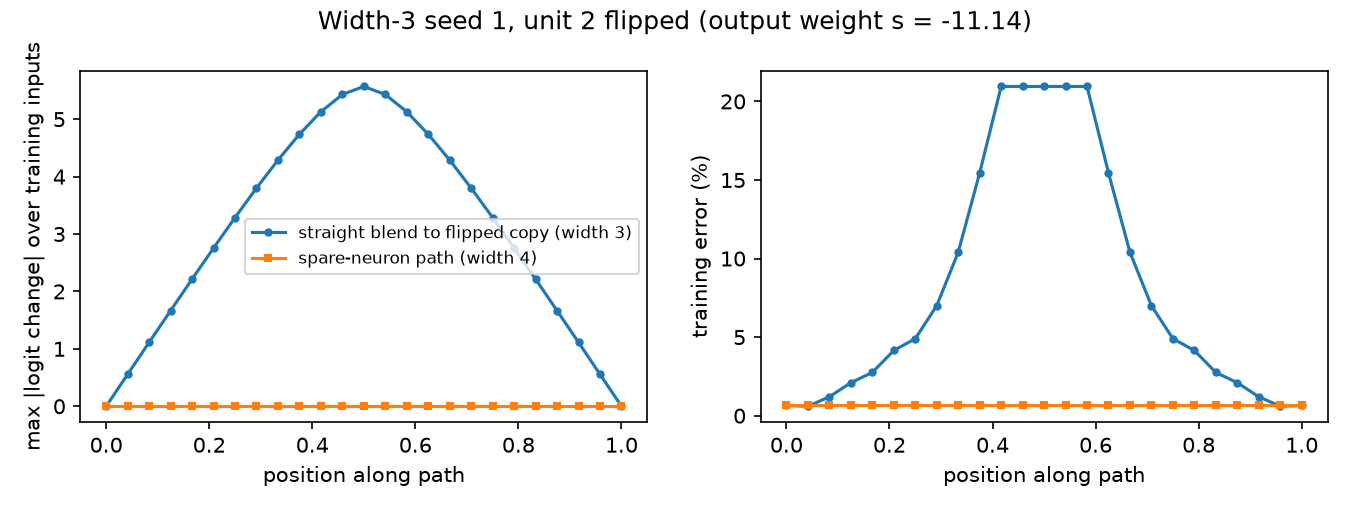
\includegraphics[width=\linewidth]{figures/b2_spare_path.png}
\caption{Width-3 network (seed 1), unit 2 flipped ($s = -11.14$). Left: largest change in the logit over the training inputs. Right: training error. Blue: straight blend to the flipped copy at width~3. Orange: the spare-neuron path of Lemma~\ref{lem:flip} at width~4, along which the function is unchanged.}
\label{fig:spare}
\end{figure}

\begin{proposition}[One spare neuron connects all permutation and sign-flip copies]
\label{prop:spare}
Let $f$ be a one-hidden-layer sigmoid network of width $r$ with an output bias, embedded in width $r+1$ by adding a unit with output weight $0$. Then each of the $2^r r!$ permutation and sign-flip copies of $f$, embedded in the same way, is joined to $f$ by a piecewise-linear path in parameter space along which the network function is exactly constant for every input. The path has at most $10r - 6$ segments if the spare unit's input parameters at the end may take any value (they do not affect the function), and at most $10r - 5$ if they must take a prescribed value, which one further segment sets. The path joins symmetry copies of one embedded network; it does not connect two independently trained networks of width $r+1$, and it does not bear on the straight-line barrier measured in Sections~\ref{sec:results} and~\ref{sec:v2}.
\end{proposition}
\begin{proof}
Three moves keep the function exactly constant along a straight segment:
\begin{itemize}[leftmargin=*]
\item[(M1)] A unit with output weight $0$ may move its input weights and bias anywhere.
\item[(M2)] Two units with identical input weights and biases may trade output weight, keeping the sum fixed, since $(a+b)\,\sigma(z)$ depends only on $a+b$.
\item[(M3)] If unit $k$ has input parameters $(-w_i, -b_i)$ and output weight $0$, then Lemma~\ref{lem:flip} moves the contribution of unit $i$ onto $k$, flipped.
\end{itemize}
Let $k$ be the spare unit. A \emph{transposition} of units $i$ and $j$ takes six segments: M1 (copy $i$'s input parameters into $k$), M2 ($i \to k$), M1 (copy $j$'s into $i$), M2 ($j \to i$), M1 (copy $k$'s into $j$), M2 ($k \to j$); the spare again has output weight zero at the end. A \emph{flip} of unit $i$ takes four: M1 (set $k$ to $(-w_i, -b_i)$), M3, M1 (copy $k$'s input parameters into $i$), M2 ($k \to i$). Any permutation of $r$ elements is a product of at most $r-1$ transpositions, and any sign pattern is a product of at most $r$ single-unit flips, so every copy is reached in at most $6(r-1) + 4r = 10r - 6$ segments.
\end{proof}

The permutation part follows the idea of Şimşek et al.~\cite{simsek2021geometry}, whose construction connects permutation copies through straight segments; the flip move M3 shifts output weight continuously between two units with opposite input parameters, which Martinelli et al.\ identify as a symmetry of constant-plus-odd activations such as the sigmoid~\cite[Appendix~A.2.2]{martinelli2024expand} (a constant-duplicate-neuron group in the terminology of Theiss et al.~\cite[Definition~B.12]{theiss2026parameter}), so Lemma~\ref{lem:flip} follows directly from their analysis. Theiss et al.\ also relate two oppositely oriented ReLU parameterizations of one function, by adjoining an auxiliary parameterization that computes the zero function rather than by a path~\cite[Example~B.13]{theiss2026parameter}. Most directly, Farrugia-Roberts proved that the functional equivalence class of any reducible single-hidden-layer $\tanh$ network is piecewise-linear path-connected~\cite[Theorem~6.1]{farrugia2023functional}; a width-$r$ network with a spare unit of output weight zero is reducible, so for $\tanh$ the existence part of Proposition~\ref{prop:spare} is his result. His construction uses a six-segment path per sign flip and a nine-segment path per transposition, and with at least half of the units blank the diameter is at most 7 segments (his Theorem~6.3); his Discussion notes that ``Future work could investigate the trade-offs between shortest path length and rank [\dots]''. Proposition~\ref{prop:spare} addresses the case with a single spare unit, for the sigmoid, with four segments per flip and six per transposition. The construction was also checked numerically on a random width-3 network with 5{,}000 random inputs, applying two transpositions and two flips: the largest change in the output along the whole path was $5.3\times10^{-15}$, and the end point equalled the target copy exactly. Two limits apply. The proposition concerns a network embedded with an inactive spare unit (output weight zero), not two independently trained networks of width $r+1$. It shows that a flat path \emph{exists}; it does not address the straight-line barrier, which is what the experiments measure. In the language of Zhao et al.~\cite{zhao2025understanding}, for an irreducible network all $2^r r!$ copies are isolated points of the set of equivalent networks at width $r$, and one extra unit joins them with an explicit curve of constant function, in the spirit of their symmetry-induced curves (Section~6.1).


\section{Weight norms and the weight-decay side-check}
\paragraph{Weight decay.} Ito et al.~\cite{ito2026permutations} report that sufficiently wide image networks (MLPs, VGG-11 and ResNet-20 widened up to 16--32$\times$) become linearly connected without permutations after temperature calibration, using weight decay 0.003 in most runs. With weaker decay ($10^{-4}$), VGG-11 and ResNet-20 show large barriers (their Section~5.4), although their Appendix~F.9 notes that ``for sufficiently wide models, smaller weight decay results in smaller barriers''. Their explanation is stated for bias-free ReLU networks with low-rank weights. The Study~1 main run used no weight decay. As a side-check with a rule dated before the run, I trained 40 width-64 networks with L2 regularization 0.003 on the weights (not the biases) added to the gradient inside Adam (not decoupled weight decay, so not a replication of any published setting). \textbf{None of the 40 networks met the inclusion rule}: all stopped at 6.15--6.80\% training error, with weights about 7 times smaller (median norm 9.4 against 66.5). With no included pairs, the dated rule gives no verdict. An exploratory comparison on all 40 networks, ignoring inclusion and decided after seeing this result, shows no clear change in the unaligned barrier (median 9.29 without decay against 14.32 with it; interval of the difference [$-1.30$, 6.68]). These networks are underfit and roughly a hundred times narrower than those of Ito et al., so this side-check does not bear on their findings.

\label{app:b4}

\begin{table}[H]
\centering
\small
\caption{Median weight norm (input and output weights, biases excluded) of included networks after 3{,}000 steps, no weight decay.}
\begin{tabular}{@{}lrrrrrrr@{}}
\toprule
Width & 3 & 4 & 6 & 8 & 16 & 32 & 64 \\
\midrule
Median norm & 32.19 & 33.69 & 38.56 & 41.02 & 46.88 & 54.96 & 66.50 \\
\bottomrule
\end{tabular}
\end{table}

\begin{table}[H]
\centering
\small
\caption{Exploratory weight-decay comparison at width 64 (all 40 networks, inclusion ignored; 20 pairs with the same initializations as the main run). Medians; interval for median(decay) $-$ median(base). Decided after seeing that no decay network met the inclusion rule.}
\begin{tabular}{@{}llrrl@{}}
\toprule
Mode & Measure & No decay & L2 0.003 & 95\% interval \\
\midrule
\md{none} & error barrier (points) & 9.29 & 14.32 & [$-1.30$, 6.68] \\
\md{none} & calibrated loss barrier & 0.197 & 0.244 & [$-0.024$, 0.074] \\
\md{wm} & error barrier (points) & 1.10 & 1.31 & [$-0.67$, 2.20] \\
\md{wm} & calibrated loss barrier & 0.023 & 0.020 & [$-0.013$, 0.016] \\
\md{wm\_sign} & error barrier (points) & 0.54 & 0.12 & [$-0.68$, 0.32] \\
\md{wm\_sign} & calibrated loss barrier & 0.010 & 0.002 & [$-0.015$, 0.001] \\
\bottomrule
\end{tabular}
\end{table}

\section{Study 2: further pre-registered outputs}
\label{app:v2more}

\begin{table}[H]
\centering\small
\caption{Study~2 Stage~1: networks meeting each inclusion threshold, by task and width (training error only; \texttt{results\_v2/stage1.csv}).}
\begin{tabular}{@{}lccccc@{}}
\toprule
Task & Width & Trained & $\le 1\%$ & $\le 2\%$ & $\le 5\%$ \\
\midrule
Coffee & 3 & 120 & 56 & 72 & 77 \\
Triangle & 2 & 100 & 0 & 0 & 0 \\
Triangle & 3 & 100 & 93 & 94 & 94 \\
Triangle & 4 & 100 & 100 & 100 & 100 \\
Triangle & 5 & 100 & 100 & 100 & 100 \\
Quadrilateral & 2 & 100 & 0 & 0 & 0 \\
Quadrilateral & 3 & 100 & 0 & 0 & 97 \\
Quadrilateral & 4 & 100 & 56 & 65 & 100 \\
Quadrilateral & 5 & 100 & 57 & 83 & 100 \\
Quadrilateral & 6 & 100 & 83 & 95 & 100 \\
Pentagon & 3 & 100 & 0 & 0 & 93 \\
Pentagon & 4 & 100 & 0 & 43 & 99 \\
Pentagon & 5 & 100 & 36 & 79 & 100 \\
Pentagon & 6 & 100 & 48 & 93 & 100 \\
Pentagon & 7 & 100 & 66 & 97 & 100 \\
Hexagon & 4 & 100 & 0 & 59 & 100 \\
Hexagon & 5 & 100 & 5 & 85 & 100 \\
Hexagon & 6 & 100 & 61 & 93 & 100 \\
Hexagon & 7 & 100 & 77 & 95 & 100 \\
Hexagon & 8 & 100 & 89 & 99 & 100 \\
\bottomrule
\end{tabular}
\end{table}

\paragraph{Flip counts.} At $h^*$ (2\%), the \md{exact\_sign} alignment flipped 0, 1, 2 and 3 units in 36, 80, 48 and 1 of the 165 pairs.

\paragraph{Widths above $h^*$ (descriptive, no claim).} Median training-error barrier, \md{wm} / \md{wm\_sign}, in points: triangle 3.37 / 0.68 (width~4) and 2.72 / 1.15 (5); quadrilateral 6.22 / 1.04 (5) and 8.23 / 1.23 (6); pentagon 4.47 / 0.10 (5), 5.11 / 0.27 (6) and 5.73 / 0.77 (7); hexagon 4.24 / 0.68 (5), 4.83 / 0.09 (6), 3.78 / 0.47 (7) and 3.76 / 0.52 (8). Above the minimal width, sign-aware matching still lowers the barrier, but it is not always removed, as in Study~1 at widths 6--64; the finite search does not cover the near-symmetries of these wider networks.

\section{Timeline of decisions}
\label{app:timeline}

\begin{table}[H]
\centering
\small
\caption{When each decision was taken. Post-hoc decisions are marked.}
\begin{tabularx}{\linewidth}{@{}lX@{}}
\toprule
Date (2026) & Decision \\
\midrule
4--5 Oct & Hypotheses H1--H3 and questions Q1--Q4 fixed and recorded, before any training \\
7 Oct & Learning-rate rule written, then checked (10 of 10 runs passed); coffee rule compared with an unofficial public copy of the lab file \\
8 Oct & Inclusion rule (2\%), line tolerances ($10^\circ$, 0.25), $\eps = 0.5$, H2 band (0.5--3), H1b distance and test; training-error barrier chosen as the deciding quantity \\
9 Oct & Main run; pre-registered verdicts written; inclusion sensitivity (1\% and 5\%); rules for the complete-group search dated before it ran \\
9--10 Oct & Complete-group search; decision not to run the signed width-8 search (post-hoc) \\
10 Oct & Weight-decay rule dated \\
11 Oct & Weight-decay run; exploratory comparison decided after the result (post-hoc); bootstrap intervals; numeric check of the draft; reproduction from a clean copy; proof of Proposition~\ref{prop:spare} \\
12 Oct & Comparison of flip counts with a fair-coin model (post-hoc); checks of numbers, code and references \\
13 Oct & Credited the flip step to Martinelli et al.\ and cited Theiss et al., after correspondence with F.~Martinelli \\
14 Oct & Citation audit: credited the existence of the spare-unit paths (for $\tanh$) to Farrugia-Roberts; cited Kanoh and Sugiyama, Wiese et al.\ and Soudry et al. \\
15 Oct & Text revisions: H3 stated as an endpoint result, sigmoid path existence inherited from $\tanh$, segment count with prescribed spare endpoint ($10r-5$), operational definition of minimal width, 25-point grid stated, inclusion counts in abstract \\
15 Oct & v2 design fixed: title rule, polygon tasks, four barrier measures, excluded-run classes \\
19 Oct & v2 rules committed (\texttt{349aa3a}) before any v2 training; Stage~1 frozen (\texttt{4c07b33}); D7 (sensitivity $h^*$) written after the training counts, before any barrier; Stage~2 run (\texttt{b7b5669}); D8 (H7 on loss) and D9 (same-line split) decided after the results (post-hoc) \\
25--26 Oct & v2.1 (text only): scope statement; flip-pair definition; construction caveat for H5; error-ceiling note; rationale for H2; mode-connectivity citations. Line-tolerance sensitivity of the same-line split (D12, post-hoc). No result changed \\
30 Oct & v2.1.2 (text only): post-hoc checks of the verdicts (pass counts with lower bounds, range of $\eps$, selection on the reported metric, inclusion, irreducibility margins; D13); H2 mis-specification and flip-count bias stated; citation pinpoints corrected. No result changed \\
30 Oct & v2.1.3 (text only): version label, deviation range, appendix cross-reference, scope of the four-measure statement, wording of two correlation results. No result changed \\
\bottomrule
\end{tabularx}
\end{table}

\end{document}
